At inference time frames come in from a live webcam feed. Each frame goes through these steps:

\begin{enumerate}
    \item \textbf{Hand Detection:} MediaPipe processes the frame and gives back per-hand landmark lists and bounding regions.
    \item \textbf{Stability Check:} Euclidean motion between frames is computed. If it's over 8 pixels, the hand is flagged unstable and we skip classification.
    \item \textbf{Crop and Pad:} The highest-confidence bounding box crop gets padded to a square using edge replication (\texttt{cv2.BORDER\_REPLICATE}). Black-border padding causes distributional shift so we avoid it.
    \item \textbf{Classification:} Crop is resized to $224 \times 224$, normalized, passed through SLD. Softmax probabilities are computed. Prediction only accepted if confidence is above 0.50.
    \item \textbf{Temporal Voting:} We maintain a majority-vote buffer of size 10. A letter only gets emitted if 70\%+ of the buffer agrees. This stops isolated mis-classifications from causing jitter.
    \item \textbf{Cooldown:} 1-second cooldown so the same letter can't fire repeatedly in quick succession.
\end{enumerate}

\subsection{FastAPI Inference Server}

The inference pipeline is exposed as a REST endpoint through a lightweight FastAPI 
\cite{fastapi} server. It takes JPEG frame uploads from any HTTP client and returns 
structured JSON.

\textbf{Endpoint:} \texttt{POST /predict} — takes a multipart-encoded JPEG and returns:

\begin{itemize}
    \item \texttt{letter} — the stable voted prediction (A--Z, \texttt{del}, \texttt{nothing}, \texttt{space}), or \texttt{null} if not yet stable.
    \item \texttt{confidence} — softmax probability of the top class.
    \item \texttt{bbox} — bounding box as $[x, y, w, h]$ in pixels.
    \item \texttt{handedness} — left or right, from MediaPipe.
    \item \texttt{motion} — Euclidean motion magnitude in pixels, used for stability gating.
    \item \texttt{landmarks} — 21 normalized landmark coords for the frontend skeleton.
    \item \texttt{error} — status string (\texttt{no hand}, \texttt{hand moving}, \texttt{low confidence}, \texttt{not stable yet}, \texttt{cooldown}) when nothing gets emitted.
\end{itemize}

Global state is managed with \texttt{threading.Lock} — prediction buffer, last emitted 
letter, cooldown timestamp all need to be thread-safe across async workers. CORS is 
open to all origins for browser access.

\begin{figure*}[!t]
    \centering
    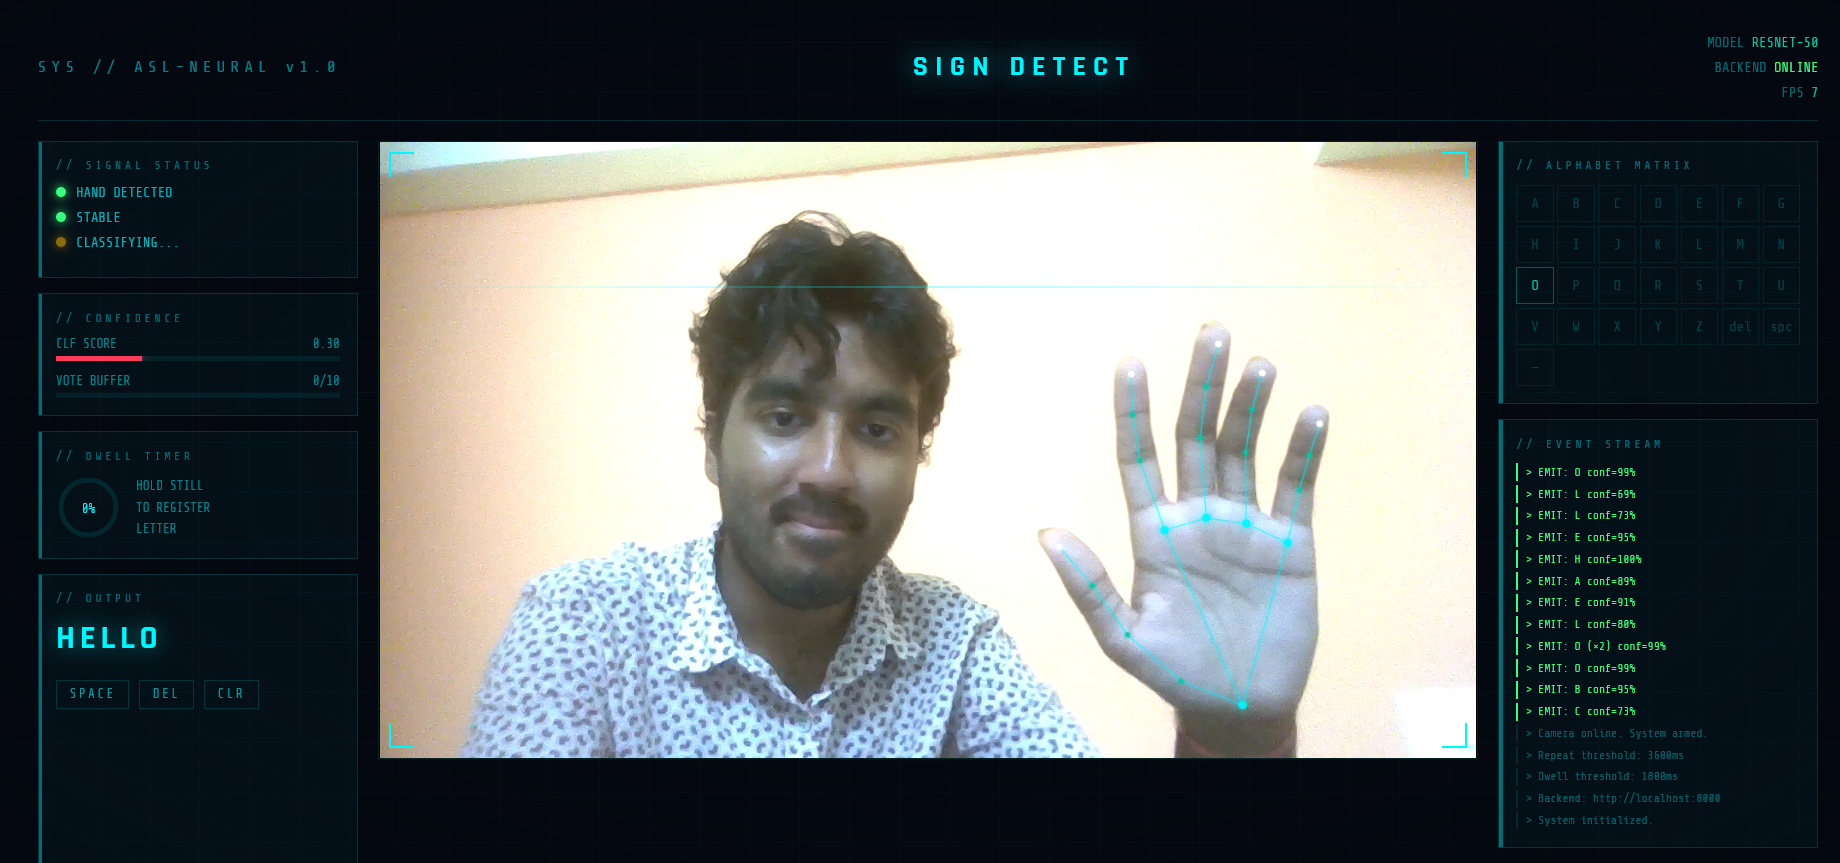
\includegraphics[width=\textwidth]{api_ss}
    \caption{FastAPI \texttt{/predict} endpoint response for a live hand frame, showing letter, confidence, bounding box, handedness, motion, and landmark fields.}
    \label{fig:api}
\end{figure*}

\subsection{Browser Frontend}

Single-page HTML/JS frontend that connects to the FastAPI server. Client-side MediaPipe 
(Tasks Vision JS SDK) runs at 60\,fps for the skeleton overlay — zero latency on that 
side. Frames are sent to the backend at around 8\,fps for actual classification. Letter 
emission uses a dwell mechanism: the prediction has to stay stable for 1.8\,s before it 
gets appended to the transcript. Repeats need 3.6\,s. Brief hand holds don't trigger 
spurious output.